\documentclass[11pt]{article}
\usepackage[utf8]{inputenc}
\usepackage{amsmath,amssymb}
\usepackage{geometry}
% hyperref omitted here so the file compiles on minimal TeX installs (hyperref pulls kvoptions).
\usepackage{graphicx}
\usepackage{xcolor}
\usepackage{caption}
\captionsetup{labelfont=bf, labelsep=period, font=small}
\usepackage{booktabs}
\usepackage{tikz}
\usetikzlibrary{positioning,arrows.meta,calc,fit,backgrounds,matrix}
\geometry{margin=1in}

% TikZ line styles: forward pass vs autograd backprop vs manual B-feedback (matches code paths)
\tikzset{
  fwd/.style={-{Stealth[length=2.4mm]}, thick, color=blue!75!black},
  bp/.style={-{Stealth[length=2.4mm]}, thick, dashed, color=violet!85!black},
  fb/.style={-{Stealth[length=2.4mm]}, thick, densely dotted, color=orange!90!black},
  box/.style={rectangle, draw=blue!40!black, rounded corners, minimum height=7mm, align=center, inner sep=3pt},
  leg/.style={font=\scriptsize, align=left}
}

\title{Feedback Matrix Models\\\large Equations and diagrams for \texttt{run\_cleanrl\_vs\_mixed\_dqn.py}}
\author{}
\date{\today}

\begin{document}
\maketitle

\begin{abstract}
This note collects the mathematical objects used in \texttt{code/run\_cleanrl\_vs\_mixed\_dqn.py}: standard CleanRL DQN, mixed backpropagation with a fixed sparse feedback matrix $B$, the $3F$-channel variant, and the five-head multi-critic with a trainable softmax mixture. We use one consistent index convention throughout and give both summation and matrix forms. Block diagrams summarize each forward pass and where TD errors inject into the linear feature layer.
\end{abstract}

% =============================================================================
\section{Index and symbol conventions}
\label{sec:indices}

\begin{itemize}
  \item \textbf{Time / transition.} At step $t$: observation vector $\mathbf{x}_t \in \mathbb{R}^{D}$ (flattened state), action $a_t \in \{0,\ldots,A-1\}$ with $A = |\mathcal{A}|$, scalar reward $r_t$, terminal flag $d_t \in \{0,1\}$, next observation $\mathbf{x}_{t+1}$.
  \item \textbf{Architecture sizes (CartPole and script defaults).} $F=120$ linear features, $H=84$ trunk hidden units, $A$ actions. The script names these \texttt{OBS\_TO\_120}, \texttt{HIDDEN\_84}.
  \item \textbf{Minibatch.} Training uses a set of sample indices $\mathcal{S}$; $B_{\mathrm{bs}} = |\mathcal{S}|$ is the batch size (\texttt{BATCH\_SIZE}${}=128$). Summations $\sum_{b \in \mathcal{S}}$ are over batch elements.
  \item \textbf{Feature / action indices.} $i \in \{0,\ldots,F-1\}$ indexes linear features $z_i$. $a,a' \in \{0,\ldots,A-1\}$ index actions. For the $3F$ variant, $j \in \{0,\ldots,K-1\}$ indexes raw output channels with $K=3F$.
  \item \textbf{Head index (multihead).} $m \in \{1,\ldots,M\}$ with $M=5$.
  \item \textbf{Matrices.} Vectors are column vectors unless stated. $\mathbf{x}^\top$ is a row; $\mathbf{u}^\top\mathbf{v}$ is a scalar inner product. $\odot$ is elementwise (Hadamard) product.
\end{itemize}

\paragraph{Discount and TD target.}
Let $\gamma \in [0,1)$ be the discount (\texttt{GAMMA}${}=0.99$). The target network is denoted by superscript ${}^{-}$. The scalar Bellman target used for all variants in this script is
\begin{equation}
\label{eq:y}
y \;=\; r + \gamma\,(1-d)\,\max_{a' \in \{0,\ldots,A-1\}} Q^{-}(\mathbf{x}_{t+1}, a').
\end{equation}
(Sometimes we write $Q(\mathbf{x},a)$ when the parameter argument is implicit.)

% =============================================================================
\section{Model I: CleanRL DQN (single MLP, full backprop)}
\label{sec:dqn}

\subsection{Forward pass (matrix form)}
Let $\theta$ collect all weights and biases. The network is
\begin{equation}
\mathbf{h}^{(1)} = \mathrm{ReLU}\!\bigl(W^{(1)}\mathbf{x} + \mathbf{b}^{(1)}\bigr) \in \mathbb{R}^{F},
\qquad
\mathbf{h}^{(2)} = \mathrm{ReLU}\!\bigl(W^{(2)}\mathbf{h}^{(1)} + \mathbf{b}^{(2)}\bigr) \in \mathbb{R}^{H},
\end{equation}
\begin{equation}
\mathbf{q} = W^{(3)}\mathbf{h}^{(2)} + \mathbf{b}^{(3)} \in \mathbb{R}^{A},
\qquad
Q(\mathbf{x},a) = q_a = \sum_{a'=0}^{A-1} \mathbf{1}[a'=a]\, q_{a'}.
\end{equation}
Here $q_a$ denotes component $a$ of $\mathbf{q}$ (0-based indexing matches the code).

\subsection{TD loss and update}
For a sampled transition $(\mathbf{x},a,r,\mathbf{x}',d)$,
\begin{equation}
\mathcal{L}_{\mathrm{TD}} = \bigl( y - Q(\mathbf{x},a) \bigr)^2
= \Bigl( y - q_a \Bigr)^2.
\end{equation}
\textbf{CleanRL DQN} minimizes $\mathcal{L}_{\mathrm{TD}}$ with Adam on \emph{all} layers; gradients flow through the entire MLP. Over a minibatch,
\begin{equation}
\mathcal{L} = \frac{1}{B_{\mathrm{bs}}} \sum_{b \in \mathcal{S}} \bigl( y^{(b)} - q^{(b)}_{a^{(b)}} \bigr)^2.
\end{equation}

\subsection{Diagram (Figure~\ref{fig:dqn})}
The subgraph is one feedforward chain. \textcolor{violet!85!black}{Dashed violet} arrows denote autograd backpropagation of $\mathcal{L}_{\mathrm{TD}}$ through \emph{all} layers. There is no separate manual $B$-feedback path.

\begin{figure}[ht]
\centering
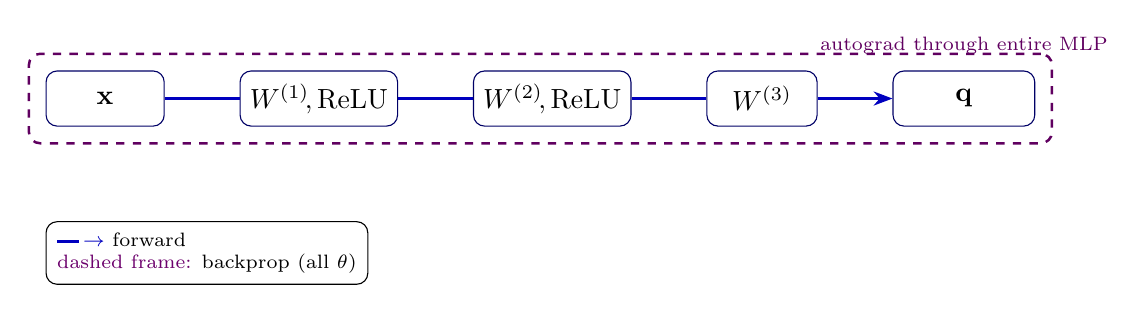
\begin{tikzpicture}[node distance=0.95cm]
\node[box, minimum width=1.5cm] (x) {$\mathbf{x}$};
\node[box, right=of x, minimum width=2.0cm] (l1) {$W^{(1)}\!,\mathrm{ReLU}$};
\node[box, right=of l1, minimum width=2.0cm] (l2) {$W^{(2)}\!,\mathrm{ReLU}$};
\node[box, right=of l2, minimum width=1.4cm] (l3) {$W^{(3)}$};
\node[box, right=of l3, minimum width=1.8cm] (q) {$\mathbf{q}$};
\draw[fwd] (x) -- (l1) -- (l2) -- (l3) -- (q);
\begin{scope}[on background layer]
  \node[draw=violet!75!black, dashed, line width=0.9pt, rounded corners=4pt, inner sep=6pt,
    fit=(x)(l1)(l2)(l3)(q)] {};
\end{scope}
\node[font=\scriptsize, text=violet!75!black, anchor=north] at ($(q.north)+(0,0.55)$) {autograd through entire MLP};
\node[draw, rounded corners, inner sep=4pt, leg, anchor=north west] at ($(x.south west)+(0,-1.2)$) {%
\textcolor{blue!75!black}{\rule[0.15em]{1em}{0.12em}\,$\rightarrow$} forward\\
\textcolor{violet!85!black}{dashed frame:} backprop (all $\theta$)};
\end{tikzpicture}
\caption{CleanRL DQN: one MLP; TD loss backpropagates through the full network.}
\label{fig:dqn}
\end{figure}

% =============================================================================
\section{Shared mixed-backprop setup (Models II and III)}
\label{sec:mixed-shared}

Split the first layer from the rest:
\begin{equation}
\mathbf{z} = W_z\,\mathbf{x} + \mathbf{b}_z \in \mathbb{R}^{F},
\qquad
\mathbf{h} = \mathrm{ReLU}\!\bigl(W_h\,\tilde{\mathbf{z}} + \mathbf{b}_h^{(1)}\bigr) \in \mathbb{R}^{H},
\end{equation}
\begin{equation}
\mathbf{h}' = \mathrm{ReLU}\!\bigl(W_{h2}\,\mathbf{h} + \mathbf{b}_h^{(2)}\bigr) \in \mathbb{R}^{H},
\qquad
\text{readout to logits (dimension depends on variant).}
\end{equation}
In code, the trunk sees $\tilde{\mathbf{z}} = \mathrm{stopgrad}(\mathbf{z})$ for the mixed updates: forward uses $\mathbf{z}$, but the TD loss gradient \emph{does not} flow into $(W_z,\mathbf{b}_z)$ via the trunk. Instead, $(W_z,\mathbf{b}_z)$ are updated by a fixed linear map $B$ applied to an error vector derived from TD error at the Q-output.

Let $\varepsilon = y - Q(\mathbf{x},a)$ be the scalar TD error for the taken action $a$. The linear-layer update uses outer products with $\mathbf{x}$; for one sample,
\begin{equation}
\label{eq:wz-update}
W_z \leftarrow W_z + \eta_z\,\boldsymbol{\delta}_z\,\mathbf{x}^\top,
\qquad
\mathbf{b}_z \leftarrow \mathbf{b}_z + \eta_z\,\boldsymbol{\delta}_z,
\end{equation}
and over a minibatch the script uses the averaged gradients
\begin{equation}
G_z = \frac{1}{B_{\mathrm{bs}}} \sum_{b \in \mathcal{S}} \boldsymbol{\delta}_z^{(b)} \bigl(\mathbf{x}^{(b)}\bigr)^\top,
\qquad
\mathbf{g}_z = \frac{1}{B_{\mathrm{bs}}} \sum_{b \in \mathcal{S}} \boldsymbol{\delta}_z^{(b)},
\end{equation}
with optional Frobenius norm clipping on $G_z$ (max norm \texttt{FEEDBACK\_GRAD\_CLIP}${}=1$), then $W_z \leftarrow W_z + \eta_z G_z$, $\mathbf{b}_z \leftarrow \mathbf{b}_z + \eta_z \mathbf{g}_z$. Learning rate $\eta_z = \texttt{LR\_LINEAR\_MIXED} = 10^{-4}$.

The trunk is trained only through $\mathcal{L}_{\mathrm{TD}} = \varepsilon^2$ with Adam at rate $\texttt{LEARNING\_RATE}=2.5\times 10^{-4}$.

% =============================================================================
\section{Model II: Mixed backprop ($B \in \mathbb{R}^{F \times A}$)}
\label{sec:mixed}

\subsection{Forward}
Same as Section~\ref{sec:mixed-shared}; the readout is $\mathbf{q} \in \mathbb{R}^{A}$ and $Q(\mathbf{x},a) = q_a$.

\subsection{Error vector and feedback}
Define $\mathbf{e} \in \mathbb{R}^{A}$ (one-hot scaled TD error):
\begin{equation}
e_{a'} = \begin{cases}
\varepsilon = y - Q(\mathbf{x},a), & a' = a,\\
0, & a' \neq a.
\end{cases}
\qquad
\text{i.e.}\quad
e_{a'} = \varepsilon\,\mathbf{1}[a'=a].
\end{equation}
Summation check: $\sum_{a'=0}^{A-1} e_{a'} = \varepsilon$.

The fixed matrix $B \in \mathbb{R}^{F \times A}$ has a single $1$ per row:
\begin{equation}
B_{i,\,a'} = \mathbf{1}\bigl[a' \equiv i \pmod{A}\bigr],
\qquad i=0,\ldots,F-1.
\end{equation}
So column $a'$ has ones in rows $i \in \{a', a'+A, a'+2A, \ldots\}$ (within range). The learning signal for features is
\begin{equation}
\label{eq:delta-z-mixed}
\boldsymbol{\delta}_z = B\,\mathbf{e} \in \mathbb{R}^{F},
\qquad
\delta_{z,i} = \sum_{a'=0}^{A-1} B_{i,a'}\, e_{a'}.
\end{equation}
Because $\mathbf{e}$ has only one nonzero entry at $a$, $\delta_{z,i} = B_{i,a}\,\varepsilon = \mathbf{1}[i \bmod A = a]\,\varepsilon$.

\paragraph{Implementation note.} In PyTorch the code computes $\boldsymbol{\delta}_z^\top = \mathbf{e}^\top B^\top$ for row batches; equivalently $\boldsymbol{\delta}_z = B\mathbf{e}$ for column $\mathbf{e}$.

\subsection{Diagram (Figure~\ref{fig:mixed})}
\textcolor{violet!85!black}{Dashed violet:} autograd from $\mathcal{L}_{\mathrm{TD}}$ through the trunk only (gradient blocked at \texttt{detach}). \textcolor{orange!90!black}{Dotted orange:} manual update $\boldsymbol{\delta}_z = B\mathbf{e}$ to $(W_z,\mathbf{b}_z)$.

\begin{figure}[ht]
\centering
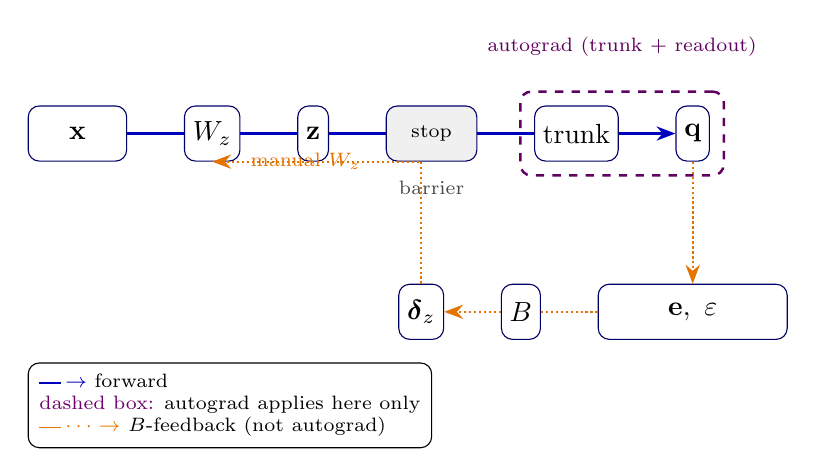
\begin{tikzpicture}[node distance=0.72cm]
\node[box, minimum width=1.25cm] (x) {$\mathbf{x}$};
\node[box, right=of x] (Wz) {$W_z$};
\node[box, right=of Wz] (z) {$\mathbf{z}$};
\node[box, right=of z, fill=gray!12, minimum width=1.15cm] (stop) {\scriptsize stop};
\node[box, right=of stop] (trunk) {trunk};
\node[box, right=of trunk] (q) {$\mathbf{q}$};
\draw[fwd] (x) -- (Wz) -- (z) -- (stop) -- (trunk) -- (q);
\begin{scope}[on background layer]
  \node[draw=violet!75!black, dashed, line width=0.9pt, rounded corners=4pt, inner sep=5pt, fit=(trunk)(q)] {};
\end{scope}
\node[font=\scriptsize, text=violet!75!black, anchor=south] at ($(trunk.north west)!0.5!(q.north east)+(0,0.5)$) {autograd (trunk + readout)};
\node[font=\scriptsize, text=gray!55!black, anchor=north] at ($(stop.south)+(0,-0.12)$) {barrier};
\node[box, below=1.55cm of q, minimum width=2.4cm] (td) {$\mathbf{e},\ \varepsilon$};
\node[box, left=of td] (B) {$B$};
\node[box, left=of B] (dz) {$\boldsymbol{\delta}_z$};
\draw[fb] (q) -- (td);
\draw[fb] (td) -- (B) -- (dz);
\draw[fb] (dz) |- node[pos=0.62, left, leg] {manual $W_z$} (Wz.south);
\node[draw, rounded corners, inner sep=4pt, leg, anchor=north west] at ($(x.south west)+(0,-2.55)$) {%
\textcolor{blue!75!black}{\rule[0.15em]{1em}{0.12em}\,$\rightarrow$} forward\\
\textcolor{violet!85!black}{dashed box:} autograd applies here only\\
\textcolor{orange!90!black}{\rule[0.15em]{1em}{0.08em}\,$\dots\rightarrow$} $B$-feedback (not autograd)};
\end{tikzpicture}
\caption{Mixed backprop ($B\in\mathbb{R}^{F\times A}$): trunk learns by autograd; $(W_z,\mathbf{b}_z)$ by $B\mathbf{e}$.}
\label{fig:mixed}
\end{figure}

% =============================================================================
\section{Model III: Mixed $3F$ ($B \in \mathbb{R}^{F \times K}$, $K=3F$)}
\label{sec:mixed3f}

\subsection{Forward: raw channels and group mean}
Let $K = 3F$. The trunk outputs $\mathbf{q}_{\mathrm{raw}} \in \mathbb{R}^{K}$. Assume $K$ divisible by $A$ and let $G = K/A$ (group size). Partition indices into action groups
\begin{equation}
\mathcal{G}_a = \{\, aG,\, aG+1,\, \ldots,\, (a+1)G - 1 \,\}.
\end{equation}
The Q-value for action $a$ is the mean over its group:
\begin{equation}
\label{eq:q3f}
Q(\mathbf{x},a) = \frac{1}{G}\sum_{j \in \mathcal{G}_a} \bigl(\mathbf{q}_{\mathrm{raw}}\bigr)_j
= \frac{1}{G}\sum_{j=0}^{K-1} \mathbf{1}[j \in \mathcal{G}_a]\,\bigl(\mathbf{q}_{\mathrm{raw}}\bigr)_j.
\end{equation}

\subsection{Error vector $\mathbf{e} \in \mathbb{R}^{K}$}
With $\varepsilon = y - Q(\mathbf{x},a)$ for the taken action $a$,
\begin{equation}
e_j = \begin{cases}
\varepsilon / G, & j \in \mathcal{G}_a,\\
0, & j \notin \mathcal{G}_a.
\end{cases}
\end{equation}
Then $\sum_{j \in \mathcal{G}_a} e_j = \varepsilon$ (sum of $G$ terms each $\varepsilon/G$).

\subsection{Feedback matrix $B \in \mathbb{R}^{F \times K}$}
For each feature $i$, average the three channels $3i, 3i+1, 3i+2$:
\begin{equation}
B_{i,j} = \begin{cases}
\frac{1}{3}, & j \in \{3i,\,3i+1,\,3i+2\},\\
0, & \text{otherwise}.
\end{cases}
\end{equation}
So
\begin{equation}
\delta_{z,i} = \sum_{j=0}^{K-1} B_{i,j}\, e_j
= \frac{1}{3}\bigl(e_{3i} + e_{3i+1} + e_{3i+2}\bigr).
\end{equation}
Matrix-vector: $\boldsymbol{\delta}_z = B\,\mathbf{e}$.

\subsection{Diagram (Figure~\ref{fig:mixed3f})}
Same legend as Figure~\ref{fig:mixed}: dashed violet box $=$ autograd through trunk and readout to $\mathbf{q}_{\mathrm{raw}}$ and pooling; dotted orange $=$ $B$-feedback to $W_z$.

\begin{figure}[ht]
\centering
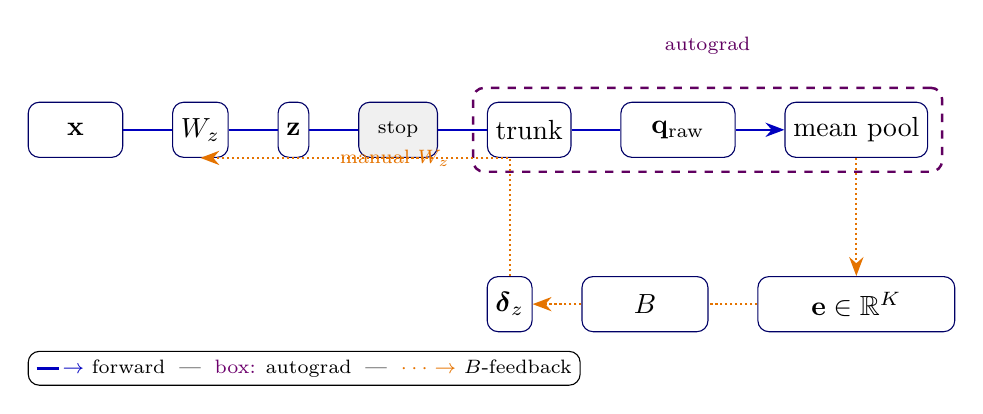
\begin{tikzpicture}[node distance=0.62cm]
\node[box, minimum width=1.2cm] (x) {$\mathbf{x}$};
\node[box, right=of x] (Wz) {$W_z$};
\node[box, right=of Wz] (z) {$\mathbf{z}$};
\node[box, right=of z, fill=gray!12, minimum width=1cm] (sg) {\scriptsize stop};
\node[box, right=of sg] (tr) {trunk};
\node[box, right=of tr, minimum width=1.45cm] (raw) {$\mathbf{q}_{\mathrm{raw}}$};
\node[box, right=of raw, minimum width=1.35cm] (pool) {mean pool};
\draw[fwd] (x) -- (Wz) -- (z) -- (sg) -- (tr) -- (raw) -- (pool);
\begin{scope}[on background layer]
  \node[draw=violet!75!black, dashed, line width=0.9pt, rounded corners=4pt, inner sep=5pt, fit=(tr)(raw)(pool)] {};
\end{scope}
\node[font=\scriptsize, text=violet!75!black, anchor=south] at ($(tr.north west)!0.5!(pool.north east)+(0,0.48)$) {autograd};
\node[box, below=1.5cm of pool, minimum width=2.5cm] (td) {$\mathbf{e}\in\mathbb{R}^K$};
\node[box, left=of td, minimum width=1.6cm] (B) {$B$};
\node[box, left=of B] (dz) {$\boldsymbol{\delta}_z$};
\draw[fb] (pool) -- (td);
\draw[fb] (td) -- (B) -- (dz);
\draw[fb] (dz) |- node[pos=0.58, left, leg] {manual $W_z$} (Wz.south);
\node[draw, rounded corners, inner sep=3pt, leg, anchor=north west] at ($(x.south west)+(0,-2.45)$) {%
\textcolor{blue!75!black}{\rule[0.15em]{1em}{0.12em}\,$\rightarrow$} forward \;|\;
\textcolor{violet!85!black}{box:} autograd \;|\;
\textcolor{orange!90!black}{$\dots\rightarrow$} $B$-feedback};
\end{tikzpicture}
\caption{Mixed $3F$: readout $\mathbb{R}^{K}$, group mean to $Q(a)$; $\boldsymbol{\delta}_z = B\mathbf{e}$ with $B\in\mathbb{R}^{F\times K}$.}
\label{fig:mixed3f}
\end{figure}

% =============================================================================
\section{Model IV: Multi-head mixed network ($M=5$ critics)}
\label{sec:multihead}

\subsection{Architecture}
Shared trunk on hidden $\mathbf{h} \in \mathbb{R}^{H}$ with five readout heads $W^{(m)} \in \mathbb{R}^{A \times H}$:
\begin{equation}
\mathbf{Q}^{(m)} = W^{(m)}\mathbf{h} + \mathbf{c}^{(m)} \in \mathbb{R}^{A},
\qquad m=1,\ldots,5.
\end{equation}
Heads $1$--$3$ use the full observation path $\mathbf{z} = W_z\mathbf{x}+\mathbf{b}_z$. Head $4$ uses $\mathbf{x}$ with pole coordinates zeroed (``cart'' mask); head $5$ uses $\mathbf{x}$ with cart coordinates zeroed (``pole'' mask). Each mask recomputes $\mathbf{z}$ through the \emph{same} $W_z$.

Trainable mixture weights $\mathbf{w} = \mathrm{softmax}(\boldsymbol{\ell}) \in \mathbb{R}^5$ with logits $\boldsymbol{\ell}$ (initialized biased toward head $1$ in code). Combined Q-values:
\begin{equation}
\label{eq:Qcomb}
Q_{\mathrm{comb}}(\mathbf{x},a) = \sum_{m=1}^{5} w_m\, Q^{(m)}(\mathbf{x},a),
\qquad
Q^{(m)}(\mathbf{x},a) = Q^{(m)}_a.
\end{equation}
The policy uses $\arg\max_a Q_{\mathrm{comb}}(\mathbf{x},a)$.

\subsection{TD targets (as in \texttt{MULTIHEAD\_UNIFIED\_TARGETS=True})}
Let $y^{(m)}$ be the Bellman target for head $m$. With unified targets, heads $1$--$3$ share the reward return target
\begin{equation}
y^{(1)} = y^{(2)} = y^{(3)} = r + \gamma(1-d)\max_{a'} Q^{(1),-}(\mathbf{x}',a'),
\end{equation}
while heads $4$ and $5$ still use masked forward paths but the same reward-based backup on their max:
\begin{equation}
y^{(4)} = r + \gamma(1-d)\max_{a'} Q^{(4),-}(\mathbf{x}',a'),
\qquad
y^{(5)} = r + \gamma(1-d)\max_{a'} Q^{(5),-}(\mathbf{x}',a').
\end{equation}
The combined head target uses the maximum over the combined Q:
\begin{equation}
y^{(\mathrm{comb})} = r + \gamma(1-d)\max_{a'} Q_{\mathrm{comb}}^{-}(\mathbf{x}',a').
\end{equation}
(If \texttt{MULTIHEAD\_UNIFIED\_TARGETS} is false, the code instead sets different $y^{(2)}, y^{(3)}$ using $\cos\theta'$ and $\gamma_{\mathrm{short}}$ on head $3$; see script.)

\medskip\noindent
Figure~\ref{fig:multihead} summarizes the forward and feedback paths: three forwards share the same $(W_z,\mathrm{trunk})$---full $\mathbf{x}$ (heads $1$--$3$), cart-masked $\mathbf{x}$ ($Q^{(4)}$), pole-masked $\mathbf{x}$ ($Q^{(5)}$). \textcolor{violet!85!black}{Dashed violet:} autograd on $\mathcal{L}$ through trunk, heads, $Q_{\mathrm{comb}}$, and $\boldsymbol{\ell}$. \textcolor{orange!90!black}{Dotted orange:} $\mathbf{e}_{\mathrm{heads}}\to B_{\mathrm{mh}}\to\boldsymbol{\delta}_z$ updates $W_z$ (with $\mathbf{z}$ stopped, autograd does not reach $W_z$).

\begin{figure}[ht]
\centering
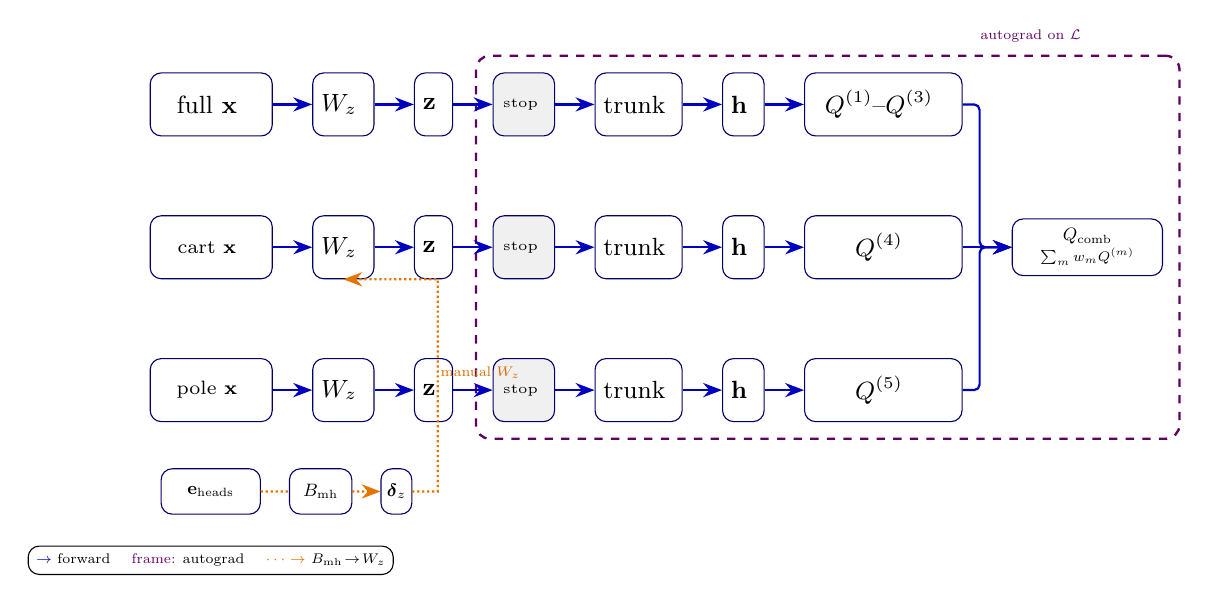
\begin{tikzpicture}[scale=0.72, transform shape, font=\small, >=Stealth]
\tikzset{
  box/.style={rectangle, draw=blue!40!black, rounded corners, minimum height=8mm, align=center, inner sep=3pt},
}
\matrix (MH) [matrix of nodes, column sep=0.5cm, row sep=1.0cm,
  nodes={box, anchor=center},
  column 1/.style={nodes={minimum width=1.55cm, font=\small}},
  column 4/.style={nodes={fill=gray!12, font=\tiny, minimum width=0.78cm}},
  column 7/.style={nodes={minimum width=2.0cm}},
] {
  full $\mathbf{x}$ & $W_z$ & $\mathbf{z}$ & stop & trunk & $\mathbf{h}$ & $Q^{(1)}$--$Q^{(3)}$ \\
  {\scriptsize cart $\mathbf{x}$} & $W_z$ & $\mathbf{z}$ & stop & trunk & $\mathbf{h}$ & $Q^{(4)}$ \\
  {\scriptsize pole $\mathbf{x}$} & $W_z$ & $\mathbf{z}$ & stop & trunk & $\mathbf{h}$ & $Q^{(5)}$ \\
};
\foreach \row in {1,2,3} {
  \foreach \col in {1,...,6} {
    \pgfmathtruncatemacro{\next}{\col+1}
    \draw[fwd] (MH-\row-\col.east) -- (MH-\row-\next.west);
  }
}
\node[box, minimum width=2.65cm, minimum height=1.0cm, align=center] (comb) at ($(MH-2-7.east)+(2.2,0)$)
  {$Q_{\mathrm{comb}}$\\[-0.08em]{\scriptsize $\sum_m w_m Q^{(m)}$}};
\draw[fwd, rounded corners=2pt] (MH-1-7.east) -- ++(0.3,0) |- (comb.west);
\draw[fwd] (MH-2-7.east) -- (comb.west);
\draw[fwd, rounded corners=2pt] (MH-3-7.east) -- ++(0.3,0) |- (comb.west);
\begin{scope}[on background layer]
  \node[draw=violet!75!black, dashed, line width=0.85pt, rounded corners=5pt, inner sep=6pt,
    fit=(MH-1-4)(MH-1-7)(MH-2-4)(MH-2-7)(MH-3-4)(MH-3-7)(comb)] {};
\end{scope}
\node[font=\scriptsize, text=violet!75!black, anchor=south west, inner sep=1pt] at ($(MH.north east)+(0.1,0.32)$) {autograd on $\mathcal{L}$};
\node[box, minimum width=1.75cm] (eh) at ($(MH.south west)+(1.25,-1.05)$) {$\mathbf{e}_{\mathrm{heads}}$};
\node[box, right=0.5cm of eh, minimum width=1.1cm] (Bm) {$B_{\mathrm{mh}}$};
\node[box, right=0.5cm of Bm] (dzm) {$\boldsymbol{\delta}_z$};
\draw[fb] (eh) -- (Bm) -- (dzm);
\coordinate (fbx) at ($(dzm.east)+(0.45,0)$);
\draw[fb] (dzm.east) -- (fbx) |- (MH-2-2.south)
  node[pos=0.28, right, font=\scriptsize, text=orange!85!black, inner sep=1pt] {manual $W_z$};
\node[draw, rounded corners, inner sep=4pt, leg, anchor=north] at ($(eh.south)+(0,-0.55)$) {%
\textcolor{blue!75!black}{$\rightarrow$} forward \quad
\textcolor{violet!85!black}{frame:} autograd \quad
\textcolor{orange!90!black}{$\dots\rightarrow$} $B_{\mathrm{mh}}\!\to\! W_z$};
\end{tikzpicture}
\caption{Multi-head ($M{=}5$): three masked pipelines; softmax-mixed $Q_{\mathrm{comb}}$; manual $B_{\mathrm{mh}}$ feedback to shared $W_z$.}
\label{fig:multihead}
\end{figure}

\subsection{Per-head TD errors and linear-layer feedback}
For each head, scalar error $\varepsilon^{(m)} = y^{(m)} - Q^{(m)}(\mathbf{x},a_t)$ with the \emph{same} sampled action $a_t$ from the replay batch. Stack $\mathbf{e}_{\mathrm{heads}} = (\varepsilon^{(1)},\ldots,\varepsilon^{(5)})^\top \in \mathbb{R}^5$.

The fixed matrix $B_{\mathrm{mh}} \in \mathbb{R}^{F \times M}$ uses the same ``one hot per row modulo $M$'' rule as \texttt{make\_fixed\_sparse\_B\_5heads}, with \emph{column} index $m \in \{0,\ldots,M-1\}$ matching the code:
\begin{equation}
(B_{\mathrm{mh}})_{i,m} = \mathbf{1}\bigl[m \equiv i \pmod{M}\bigr],
\qquad i=0,\ldots,F-1,\ m=0,\ldots,M-1.
\end{equation}
Stack head errors as $\mathbf{e}_{\mathrm{heads}} = (\varepsilon^{(1)},\ldots,\varepsilon^{(5)})^\top$ (heads numbered as in the code). Then
\begin{equation}
\boldsymbol{\delta}_z = B_{\mathrm{mh}}\,\mathbf{e}_{\mathrm{heads}},
\qquad
\delta_{z,i} = \sum_{m=0}^{M-1} (B_{\mathrm{mh}})_{i,m}\,\varepsilon^{(m+1)}.
\end{equation}
(Equivalently: map head index $h\in\{0,\ldots,4\}$ to column $m=h$ so $\delta_{z,i}=\varepsilon^{(i \bmod M + 1)}$ when each row has a single nonzero.)

\subsection{Loss}
\begin{equation}
\mathcal{L}_{\mathrm{heads}} = \sum_{m=1}^{5} \bigl( y^{(m)} - Q^{(m)}(\mathbf{x},a_t) \bigr)^2,
\qquad
\mathcal{L}_{\mathrm{comb}} = \bigl( y^{(\mathrm{comb})} - Q_{\mathrm{comb}}(\mathbf{x},a_t) \bigr)^2,
\end{equation}
\begin{equation}
\mathcal{L} = \mathcal{L}_{\mathrm{heads}} + \lambda_{\mathrm{mh}}\,\mathcal{L}_{\mathrm{comb}},
\qquad \lambda_{\mathrm{mh}} = \texttt{MULTIHEAD\_COMBINED\_LOSS\_WEIGHT} = 2.
\end{equation}
Adam updates \emph{all} parameters (including $\boldsymbol{\ell}$) on $\mathcal{L}$; the linear layer \emph{also} receives the manual $B_{\mathrm{mh}}$ update as in \eqref{eq:wz-update}, with trunk forward using $\mathrm{detach}(\mathbf{z})$ for the TD part that drives $\mathcal{L}$ (same pattern as other mixed variants).

% =============================================================================
\section{Equivalence checklist (diagrams $\leftrightarrow$ code)}
\label{sec:check}

\begin{itemize}
  \item \textbf{DQN:} Equation~\eqref{eq:y} with single $\mathbf{q}$ match \texttt{CleanRLQNetwork} and MSE on gathered $q_a$.
  \item \textbf{Mixed:} $\boldsymbol{\delta}_z = B\mathbf{e}$ with one-hot $\mathbf{e}$ matches \texttt{delta\_z = e @ B\_fixed.t()}; manual $W_z$ update matches \texttt{linear\_feature.weight.data.add\_}.
  \item \textbf{$3F$:} Group mean \eqref{eq:q3f} matches \texttt{q\_from\_raw}; spread of $\varepsilon/G$ on $\mathcal{G}_a$ matches \texttt{spread[action]}; $B_{i,3i+k}=1/3$ matches \texttt{make\_fixed\_sparse\_B\_3f}.
  \item \textbf{Multihead:} Softmax mixture \eqref{eq:Qcomb} matches \texttt{F.softmax(self.weight\_logits)}; $B_{\mathrm{mh}}$ matches \texttt{make\_fixed\_sparse\_B\_5heads}; stacked errors match \texttt{e = torch.cat([e1,\ldots,e5], dim=1)}.
\end{itemize}

% =============================================================================
\section{Comparison}
\label{sec:compare}

\begin{table}[ht]
\centering
\caption{How each architecture trains the linear feature layer $W_z$ vs.\ the trunk (readout).}
\label{tab:compare}
\resizebox{\linewidth}{!}{%
\small
\setlength{\tabcolsep}{6pt}
\begin{tabular}{@{}lcccp{3.5cm}@{}}
\toprule
\textbf{Model} & \textbf{Autograd to $W_z$?} & \textbf{Manual $B$ to $W_z$?} & \textbf{Trunk} & \textbf{Feedback shape} \\
\midrule
CleanRL DQN & yes & no & full MLP & --- \\
Mixed ($A$) & no & yes ($B\in\mathbb{R}^{F\times A}$) & trunk + readout & one-hot TD on $a$ \\
Mixed $3F$ & no & yes ($B\in\mathbb{R}^{F\times K}$) & trunk + $K$-dim readout & spread TD on group $\mathcal{G}_a$ \\
Multihead & no & yes ($B_{\mathrm{mh}}\in\mathbb{R}^{F\times 5}$) & shared trunk + 5 heads + softmax & stacked head errors \\
\bottomrule
\end{tabular}%
}
\end{table}

The table contrasts how $W_z$ is trained: only mixed variants (including multi-head, Figure~\ref{fig:multihead}) use manual $B$-feedback; CleanRL DQN relies on autograd into $W_z$ through the full MLP.

\end{document}
